\addcontentsline{toc}{subsection}{\textit{n}th-Term Test for Divergence}
\subsection*{\textit{n}th-Term Test for Divergence}
\begin{tcolorbox}[title= LIMIT OF THE nTH TERM OF A SERIES,colframe=black,sharp corners,colback=white,colbacktitle=white,coltitle=black]

    \begin{center}
    Let $\displaystyle\sum a_n$ converge, then $\displaystyle\lim_{n\to\infty}a_n=0$.
    
    
    If $\displaystyle\lim_{n\to\infty}a_n\ne0$, then $\displaystyle\sum a_n$  diverges.
    \end{center}
    
\end{tcolorbox}
We commonly abbreviate the name of this theorem to the "Divergence Test".\\
\\
\noindent\textbf{Example: Using the Divergence Test}\\
Determine the convergence or divergence of each series.
\begin{parts}
    \begin{minipage}{0.23\linewidth}
        \part $\displaystyle\sum_{n=0}^{\infty}2^n$
    \end{minipage}
    \hfill
    \begin{minipage}{0.23\linewidth}
        \part $\displaystyle\sum_{n=1}^{\infty}\frac{n!}{2n!+1}$
    \end{minipage}
    \hfill
    \begin{minipage}{0.23\linewidth}
        \part $\displaystyle\sum_{n=1}^{\infty}\frac{1}{n}$
    \end{minipage}
    \vspace{\stretch{1}}
\end{parts}

\noindent\textbf{Example: Bouncing Ball Problem}\\
A ball is dropped from a height of 6 feet and begins bouncing as shown in the figure below. The height of each bounce is three-fourths the height of the previous bounce. Find the total vertical distance traveled by the ball.


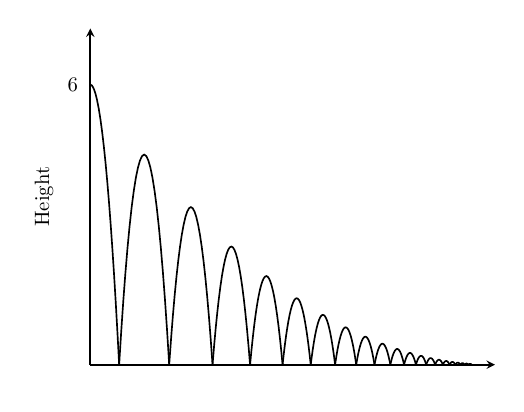
\begin{tikzpicture}[scale=.75,
  declare function={
    bounce(\hz,\idx) = \hz*(3/4)^\idx;
    duration(\hz,\idx) = sqrt(2*\hz/9.81)*(1+sqrt(3)*(1-sqrt(3/4)^\idx)/(1-sqrt(3/4)));
    offset(\hz,\idx) = duration(\hz,\idx-1)+(duration(\hz,\idx)-duration(\hz,\idx-1))/2;
    flight(\hz,\idx,\t) = bounce(\hz,\idx)-9.81/2*(\t-offset(\hz,\idx))^2;
  }
]
  \begin{axis}[
      xmin=0, xmax=20,
      ymin=0, ymax=12,
      thick,
      axis lines=left,
      xtick={14.047},
      ytick={10},
      %xtick={{duration(10,8)}},
      xticklabels={},
      yticklabels={6},
      xlabel={},
      ylabel={Height},
      tick style=transparent,
  ]
    \addplot[domain=0:{duration(20,0)}] {bounce(10,0)-9.81/2*\x^2};
    \foreach \p in {1,...,20} {
      \addplot[domain={duration(10,\p-1)}:{duration(10,\p)}] {flight(10,\p,\x)}; 
    }
    
  \end{axis}
\end{tikzpicture}

\vspace{\stretch{1}}




\newpage
